\documentclass[tikz,border=4pt]{standalone}
\usepackage{amsmath,amssymb}

\usetikzlibrary{arrows.meta,positioning,automata,shapes,shapes.misc,calc,decorations.pathmorphing,decorations.markings,angles,quotes,patterns,mindmap,matrix,knots,hobby,trees}
\tikzset{->-/.style={decoration={markings, mark=at position 0.5 with {\arrow{Stealth}}}, postaction={decorate}}}
\begin{document}
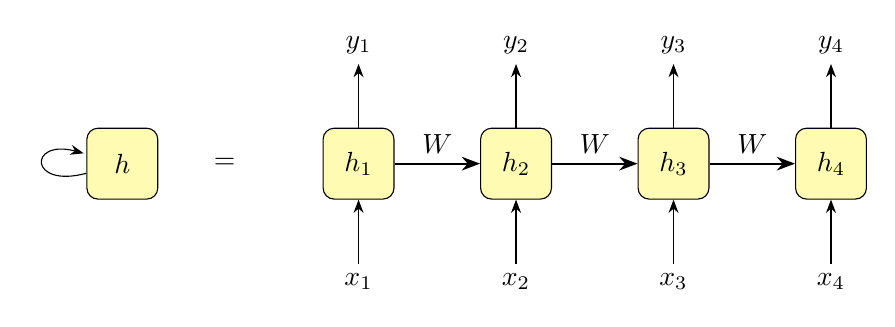
\begin{tikzpicture}[b/.style={draw, rounded corners, fill=yellow!30, minimum size=9mm}, >=Stealth]
\foreach \t in {1,...,4} {
  \node[b] (h\t) at (2*\t,0) {$h_\t$};
  \node (x\t) at (2*\t,-1.5) {$x_\t$};
  \node (y\t) at (2*\t,1.5) {$y_\t$};
  \draw[->] (x\t) -- (h\t); \draw[->] (h\t) -- (y\t);
}
\foreach \t [count=\s from 2] in {1,...,3} \draw[->, thick] (h\t) -- node[above] {$W$} (h\s);
\node[b] (h) at (-1,0) {$h$}; \draw[->] (h) edge[loop left] (h); \node at (0.3,0) {$=$};
\end{tikzpicture}
\end{document}
